\documentclass[]{article}
\usepackage{lmodern}
\usepackage{graphicx}
\usepackage{fancyhdr}
\pagestyle{fancy}
\rhead{Specyfikacja funkcjonalna w Javie: jaguar}
\usepackage{amssymb,amsmath}
\usepackage[utf8]{inputenc}
\usepackage[english]{babel}
\usepackage{lastpage}
\usepackage{amsmath,amscd}
\usepackage[all,cmtip]{xy}
\usepackage{ifxetex,ifluatex}
\usepackage{fixltx2e} % provides \textsubscript
\ifnum 0\ifxetex 1\fi\ifluatex 1\fi=0 % if pdftex
  \usepackage[T1]{fontenc}
  \usepackage[utf8]{inputenc}
\else % if luatex or xelatex
  \ifxetex
    \usepackage{mathspec}
  \else
    \usepackage{fontspec}
  \fi
  \defaultfontfeatures{Ligatures=TeX,Scale=MatchLowercase}
\fi
% use upquote if available, for straight quotes in verbatim environments
\IfFileExists{upquote.sty}{\usepackage{upquote}}{}
% use microtype if available
\IfFileExists{microtype.sty}{%
\usepackage[]{microtype}
\UseMicrotypeSet[protrusion]{basicmath} % disable protrusion for tt fonts
}{}
\PassOptionsToPackage{hyphens}{url} % url is loaded by hyperref
\usepackage[unicode=true]{hyperref}
\hypersetup{
            pdftitle={Specyfikacja funkcjonalna generatora i analizatora grafów: jaguar},
            pdfauthor={Kuźmicki Maciej, Skiba Szymon},
            pdfborder={0 0 0},
            breaklinks=true}
\urlstyle{same}  % don't use monospace font for urls
\usepackage{multicol}
\IfFileExists{parskip.sty}{%
\usepackage{parskip}
}{% else
\setlength{\parindent}{0pt}
\setlength{\parskip}{6pt plus 2pt minus 1pt}
}
\setlength{\emergencystretch}{3em}  % prevent overfull lines
\providecommand{\tightlist}{%
  \setlength{\itemsep}{0pt}\setlength{\parskip}{0pt}}
\setcounter{secnumdepth}{0}
% Redefines (sub)paragraphs to behave more like sections
\ifx\paragraph\undefined\else
\let\oldparagraph\paragraph
\renewcommand{\paragraph}[1]{\oldparagraph{#1}\mbox{}}
\fi
\ifx\subparagraph\undefined\else
\let\oldsubparagraph\subparagraph
\renewcommand{\subparagraph}[1]{\oldsubparagraph{#1}\mbox{}}
\fi
% set default figure placement to htbp
\makeatletter
\def\fps@figure{htbp}
\makeatother
\title{Specyfikacja funkcjonalna generatora i analizatora grafów: \texttt{jaguar}}
\author{Kuźmicki Maciej, Skiba Szymon}
\date{09.03.2022}
\begin{document}
\maketitle
\thispagestyle{fancy}
\section{Cel projektu}\label{header-n231}
\cfoot{Page \thepage \hspace{1pt} of \pageref{LastPage}}
Program \texttt{jaguar} ma na celu tworzenie oraz analizowanie grafów i dróg pomiędzy wierzchołkami. 
Program działa w trybie interaktywnym z graficznym interfejsem użytkownika. Użytkownik ma w nim możliwość generowania grafu w trzech trybach oraz wczytywania do programu grafu z pliku o odpowiednim formacie, jak również zapisywanie wygenerowanego grafu do pliku. Ponadto, program będzie wyświetlał informację o tym, czy wczytany graf jest spójny, natomiat żeby uzyskać najkrótszą odległość pomiędzy dwoma wierzchołkami należy w odpowiednim do tego miejscu podać wierzchołek startowy oraz końcowy, bądź wskazać te wierzchołki za pomocą myszki. Program powinien wyświetlić najkrótszą trasę na ekranie oraz podać wartość liczbową tej trasy. Generowany i analizowany graf będzie zawsze miał formę prostokąta o liczbie wierzchołków równej \verb|liczba_wierszy*liczba_kolumn|,  gdzie wierzchołki będą numerowane od 0 wierszami.

\section{Dane wejściowe i wyjściowe}\label{header-n233}
Wszystkie informację dotyczące danych wejściowych, jak i wyjściowych, które będzie przetrwarzał program znajdują się poniżej:
\begin{itemize}
\item
Program \texttt{jaguar} będzie miał możliwość wczytania grafu z pliku o odpowiednim formacie, jak i zapisania wygenerowanego grafu do pliku. W pierwszej linijce powinna znaleźć się liczba wierszy oraz kolumn oddzielona pojedyńczą spacją. Natomiast w kolejnych linijkach pliku powinny znaleźć się numery wierzchołków sąsiadujących z wierzchołkiem o numerze \texttt{n-1}, gdzie \texttt{n} jest numerem aktualnej linijki pliku zawierającego graf, wraz z ich wagami. Reprezentacja takiego grafu znajduję się na rysunku nr 1, jest to jednak jedynie zdjęcie poglądowe, aby zrozumieć, w jakiej formie przechowywane są informacje. Powinny one zostać zapisane w poniższy sposób:


\texttt{2 3\\
1 :0,88435  3 :1,3444\\
0 :1,12121  2 :0,2342  4 :1,2111\\
1 :0,76883  5 :0,2883\\
0 :0,79887  4 :1,3496\\
1 :1,76344  3 :1,8677  5 :0,1323\\
2 :1,12312  4 :1,2932}

Po wczytaniu grafu z pliku, bądź zapisaniu grafu do pliku program wyświetli komunikat o tym, czy dana operacja się powiodła. 

\begin{equation*}
\xymatrix@C=3cm{
  0 \ar[r]|{0,88435} \ar@<-2pt>[d]_{1,3444} & 1 \ar@<-2pt>[d]_{1,21111} \ar[r]|{0,2342}\ar@<-6pt>[l]|{1,12121} & 2 \ar@<-4pt>[d]_{0,2883}\ar@<-6pt>[l]|{0,76883}\\
   3\ar@<-2pt>[u]_{0,79887} \ar[r]|{1,3496}   & 4 \ar@<-2pt>[u]_{1,76344} \ar@<-0pt>[r]|{0,1323} \ar@<-6pt>[l]|{1,8677} & 5 \ar@<-6pt>[l]|{1,2932} \ar@<-2pt>[u]_{1,12312}
}
\end{equation*}
\begin{center}
(rys. 1)
\end{center}
\item
W celu wygenerowania grafu zawierającego wszystkie możliwe krawędzie pomiędzy dowolnymi dwoma sąsiadami, grafu spójnego, bądź grafu losowego program \texttt{jaguar} będzie miał na górze możliwość wybrania jednego z trzech trybów, natomiast obok znajdzie się okienko w którym możemy podać zakres wag, z których program będzie losował wagi.
Wagi te muszą być liczbami rzeczywistymi dodatnimi.
\item
Program \texttt{jaguar} po wczytaniu pliku będzie w okienku na górze wyświetli informację o tym, czy wczytany graf jest spójny, nie będzie potrzeby klikania żadnej opcji, program domyślnie sprawdzi spójność grafu.
\item
W kolejnym okienku na górze będzie możliwość podania indeksów dwóch wierzchołków (wierzchołka początkowego i końcowego) pomiędzy którymi ma zostać wyznaczona najkrótsza droga. Kolejną możliwością będzie zaznaczenie myszką na wizualizacji grafu odpowiednich wierzchołków. Program w obu wypadkach zaznaczy na obrazku najkrótszą drogę oraz wyświetli komunikat o łącznej wadze przebytej drogi.

\end{itemize}

\section{Interfejs graficzny użytkownika}\label{header-n256}
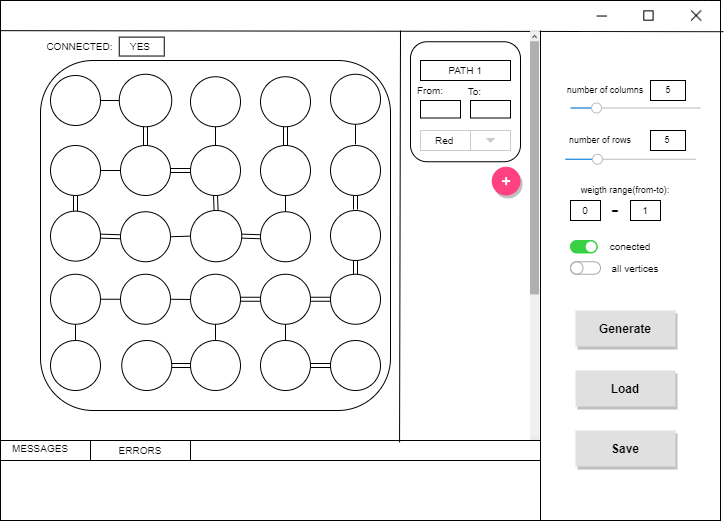
\includegraphics[scale=0.5]{gui_jimp.drawio}
\begin{center}
(rys. 2 Projekt GUI)
\end{center}
\texttt
GUI będzie w postaci desktopowej aplikacji okienkowej. Wielkość okna będzie można zmniejszać i ukrywać za pomocą górnego paska z opcjami : zamknij, rozszerz i minimalizuj. W prawej części interfejsu znajdują się suwaki do dostosowania wielkości grafu i jego parametrów oraz trzy przyciski służące do generowania grafu (zgodnie z ustawionymi parametrami); wczytywania grafu (parametry po wczytaniu odpowiednio się zaktualizują); zapisywania. W dolnej części znajduje się okno dialogowe ("| MESSAGES | ERRORS |") które wyświetla odpowiednie informacje o wykonanych działaniach i wiadomości o błędach. Główną część okna zajmuje wyświetlacz grafu. Graf jest przedstawiony za pomocą kropek i połączeń dwustronnych lub pojedynczych, po kliknięciu na takie połączenie wyświetla się jego waga i kierunek. Ścieżki w grafie można wybierać klikając prawym przyciskiem myszy na wierzchołek lub dodawać je za pomocą plusa w segmencie po prawej od grafu. Wszystkie ścieżki wyświetlają się w segmencie po prawej i dostępny jest suwak w zależności od ich ilości. Wielkość grafu i kropek skaluje się odpowiednio wraz z wzrostem krawędzi i rzędów.




\section{Teoria}\label{header-n279}

Program będzie korzystał z algorytmu BFS do przeszukiwania grafu wszerz po to, by sprawdzić czy jest on spójny. Grafy spójne będą generowane metodą bruteforce generując losowe grafy aż do otrzymania grafu spójnego. Do znajdowania najkrótszej drogi pomiędzy dowolnymi dwoma wierzchołkami zostanie wykorzystany algorytm Dijkstry. Do przechowywania grafu w pamięci komputera zostanie wykorzystana lista sąsiedztwa przechowująca informacje o sąsiadach kolejnych wierzchołków wraz z wagami przejścia pomiędzy nimi. 



\section{Komunikaty błędów}\label{header-n281}

\begin{itemize}
\item
  \texttt{BŁĄD\ 1:\ Nie\ udało\ się\ przeczytać\ pliku.\ Nieprawidłowy\ format\ pliku.}

  Gdy wczytywany plik będzie zawierał niewłaściwy format danych wejściowych program wyświetli komunikat o błędzie oraz zignoruje ten plik.
\item
  \texttt{BŁĄD\ 2:\ Podano\ nieistniejące\ wierzchołki\ grafu\ do\ obliczenia\ odległości\ pomiędzy\ nimi.}

 Gdy do obliczenia odległości pomiędzy dwoma wierzchołkami grafu podamy indeks wierzchołka, który wychodzi poza zakres naszego grafu program wyświetli komunikat o błędzie oraz zignoruje podane dane wejściowe.


\end{itemize}

\end{document}